\chapter{Iteración 5}
\section{Objetivos de iteración}
\begin{itemize}
  \item Implementación inicial de API REST
  \item Primeros tests
  \item Despliegue en plataforma Azure
  \item Investigar integración contínua
\end{itemize}


\section{Implementación inicial de API REST}
Hemos definido un primer borrador del API REST a implementar por el servidor. No
es una especificación exhaustiva o completa pero las partes aún no determinadas
de la misma necesitan de información aún no disponible (como por ejemplo las 
necesidades concretas de filtrado de los clientes del servidor).

En siguientes iteraciones queremos integrar la documentación generada por
\emph{Swagger} al final de la memoria. Mientras tanto documento aquí el
borrador actual de la especificación de la API y su implementación actual.

\subsection{API}
El API tiene dos puntos de entrada: \texttt{sessions} y \texttt{session}. 

Todos los recursos responden con contenido \texttt{application/json} con
codificación \texttt{UTF-8}. Los códigos de respuesta HTTP serán siempre
2xx para peticiones correctas, 4xx para errores en la petición y 5xx cuando
hay un error en el servidor.

Toda petición debe incluir dos cabeceras específicas de \emph{GameRegistry}
donde se comunique el identificador de usuario y su token tal y como lo 
validó/generó el \emph{Servidor de Login} del sistema distribuido. Ambos
parámetros serán validados por \emph{GameRegistry} contra el 
\emph{Servidor de Login}.

\subsubsection{/sessions}
Representa una colección de sesiones de juego. Métodos HTTP:

\begin{itemize}
 \item \textbf{GET}: Devuelve una colección de sesiones de juego. Debe aceptar
       parámetros que permitan filtrar la colección. Los parámetros aún no han
       sido definidos (a la espera de conocer las necesidades de los clientes 
       de \emph{GameRegistry}). Devolverá \texttt{200 OK} y una colección de
       sesiones si tiene éxito.
 \item \textbf{POST}: Añade una nueva sesión de juego a la colección. Devolverá
       \texttt{201 Created} si tiene éxito.
 \item \textbf{PUT}: En una especificación REST el comando PUT significa 
       \emph{reemplazar} el recurso con otro. Dicha operación no debe permitirse
       en este contexto por lo que \emph{GameRegistry} devolverá ante peticiones
       como esta el código \texttt{405 Method Not Allowed}.
 \item \textbf{DELETE}: Al igual que PUT, el servidor no debe permitir borrar toda
       la colección de sesiones. Devolverá \texttt{405 Method Not Allowed}.
\end{itemize}

\subsubsection{/sessions/:id}
Representa una única session de juego determinada por su identificador (\texttt{id}). 
Métodos HTTP:

\begin{itemize}
 \item \textbf{GET}: Devuelve la sesión de juego identificada por \texttt{id} con
       código HTTP \texttt{200 OK}. Si no hay sesión con dicho \texttt{id} entonces
       devolverá \texttt{404 Not Found}.
 \item \textbf{POST}: En una especificación REST este comando significa 
       \emph{añadir una nueva entrada a la colección} pero la URL 
       \texttt{/session/:id} no representa una colección sino una única sesión de juego.
       Por tanto este método no tiene sentido y el servidor devolverá 
       \texttt{405 Method Not Allowed}.
 \item \textbf{PUT}: Reemplaza la sesión de juego por la nueva sesión suministrada
       en la petición. Devolverá \texttt{200 OK} o \texttt{404 Not Found} si no hay
       ninguna sesión con ese identificador.
 \item \textbf{DELETE}: Elimina la sesión de juego con el identificador dado. Devolverá
       \texttt{204 No Content} si tiene éxito o \texttt{404 Not Found} si no encuentra
       la sesión de juego.
\end{itemize}

\subsubsection{Otros}
Es muy posible que los requerimientos de los sistemas que dependen de \emph{GameRegistry}
obliguen a implementar nuevos puntos de entrada con comportamientos específicos.


\section{Primeros tests}
Hemos comenzado a escribir una batería de tests automáticos que comprueben el correcto
funcionamiento del servidor.

Los tests incluidos son:

\begin{itemize}
 \item \texttt{testNotFound}: Busca una sesión inexistente, comprueba resultado.
 \item \texttt{testCreate}: Crea una nueva sessión.
 \item \texttt{testUpdate}: Crea una sesión, sube una nueva versión.
 \item \texttt{testDelete}: Crea una sesión, la borra , comprueba que no existe a continuación.
 \item \texttt{testFindSessions}: Crea una sesión y después la busca y comprueba el contador de resultados.
 \item \texttt{testNotAuthenticated}: Intenta una petición sin especificar usuario y token, comprueba error.
\end{itemize}



\section{Despliegue en plataforma Azure}
Tras evaluar las opciones de despliegue de \emph{Docker} en \emph{Azure} hemos
optado por construir una máquina virtual donde administraremos manualmente una
instancia de \emph{Docker} en vez de utilizar la extensión de máquina virtual
que implementa \emph{Azure} para \emph{Docker}. Utilizar esta última habría implicado
una complejidad añadida por la parafernalia necesaria para mantener certificados de
seguridad para poder comunicarnos con la instancia de  \emph{Docker}.

En lugar de la extensión de máquina virtual de \emph{Azure} administraremos la 
máquina virtual manualmente.


\subsection{Test vm}
Para esta iteración hemos creado una máquina virtual cuyo propósito es familiarizarnos
con el entorno \emph{Azure}. Para ello los requisitos de esta máquina serían:

\begin{itemize}
 \item Ser capaz de ejecutar el servidor \emph{GameRegistry} y \emph{MongoDB} como
       contenedores de \emph{Docker}.
 \item Ser capaz de construir el contenedor de \emph{GameRegistry} a partir del 
       repositorio SVN del proyecto.
\end{itemize}

Para ello se ha basado la máquina virtual en una imagen de \emph{Ubuntu 15.04}, que contiene
una versión reciente y razonablemente testada de \emph{Docker}. Además hemos añadido
el cliente de \emph{Subversion} y el \emph{OpenJDK-8}.


\subsection{VM de producción}
Aún no creada. Sus requisitos son similares pero no iguales a la máquina test. El propósito
de esta máquina virtual será el de ejecutar el servidor, evitando la instalación
de cualquier pieza de software no necesaria para esa tarea, lo cual en este caso implica
no instalar ningún \emph{JDK} ni \emph{Subversion}.

Esto requiere algún método para hacer llegar el contenedor con el servidor GameRegistry a
la máquina que no implique a \emph{Subversion} ni el uso de \emph{Java} para compilar
el código fuente. Lo resolveremos en la próxima iteración.

\begin{figure}[h]
 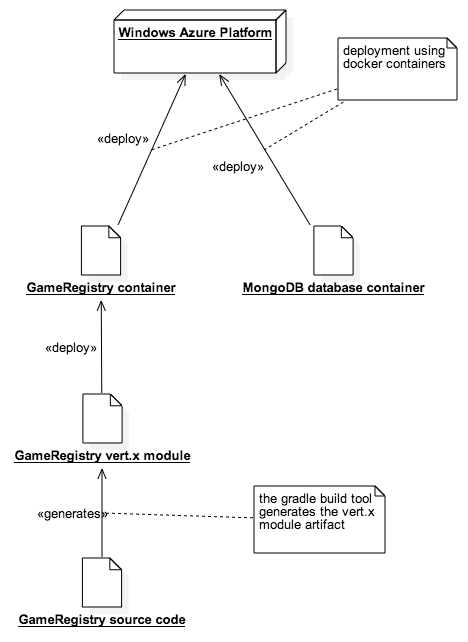
\includegraphics[scale=0.6]{diagrams/docker_deployment_diagram.png}
 \caption{Diagrama de despliegue (iteración 5)}
 \label{fig:despliegue}
\end{figure} 


\section{Investigar integración contínua}
Algún método de integración contínua sería interesante para el proyecto de forma que los tests 
sean ejecutados en cada revisión del proyecto. Hay sitios web que ofrecen una instancia gratuita de
integración contínua que podrían ser utilizados, como por ejemplo:

\begin{itemize}
\item CircleCI (\texttt{https://circleci.com/})
\item CodeShip (\texttt{https://codeship.com/})
\end{itemize}

Estamos aún estudiando la viabilidad y los requisitos impuestos por dichas opciones.